\documentclass{standalone}
\usepackage{pgfplots}
\usepackage{siunitx}
\usepackage[dvipsnames]{xcolor}

\pgfplotsset{compat=1.18}

\begin{document}
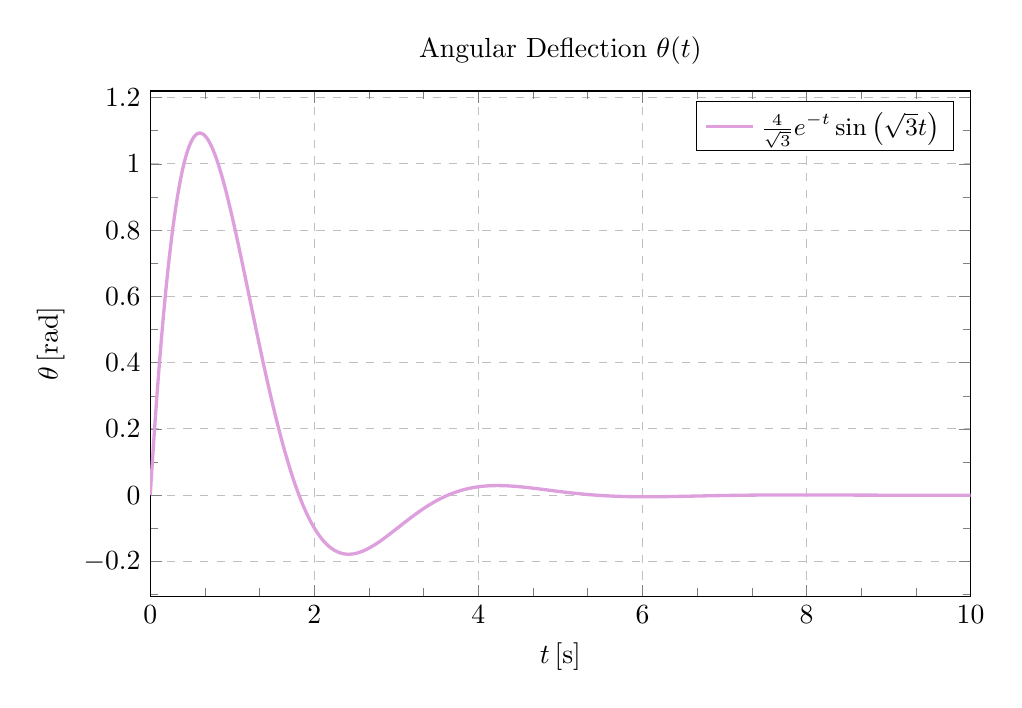
\begin{tikzpicture}
	\begin{axis}[
		title={Angular Deflection \( \theta(t) \)},
		width=12cm,
		height=8cm,
		xlabel={\(t \, [\si{\second}]\)},
		ylabel={\(\theta \, [\si{\radian}]\)},
		grid=major,
		grid style=dashed,
		samples=1000,
		legend style={font=\small},
		domain=0:10,
		xmin=0,
		xmax=10,
		xtick distance=2,
		minor x tick num=2,
		ytick distance=0.2,
		minor y tick num=1,
	]
	\addplot[
		color=Plum,
		line width=1.2pt,
	] {4 *exp(-x)*sin(deg(sqrt(3)*x))/sqrt(3)};
	\addlegendentry{\( \frac{4}{\sqrt{3}} e^{-t} \sin{\left( \sqrt{3}t \right)} \)}
	\end{axis}
\end{tikzpicture}

\end{document}
